
\chapter{Additional Features}
\setcounter{figure}{0}
\setcounter{table}{0}

\label{sec:AdditionalFeatures}
\section{OptimumTire Add-in}
\label{sec:OptimumTAddin}

The OptimumTire add-in allows users to access all of the output quantities in OptimumTire from Excel, Matlab or any other software package that supports COM components. Simulations and calculations that require a tire model can be done easily using this feature. Look-up tables of the tire charactereistics can also be created quickly for use in other applications. 

In the add-in, the model coefficients are specified to the OptimumTire functions with long character strings. These strings can be directly exported from OptimumTire. To do this first click on the desired tire model in the project tree. This will expose the model coefficients in the data entry area. Then click on the \textit{Options} button as shown in Figure~\ref{fig:AddinExport}. Then select \textit{Export} and \textit{Add-in Model to Clipboard}. This will copy the encoded string to the computer clipboard and allow it to be pasted into Excel or any other software.

\begin{figure}[H]
	\centering
		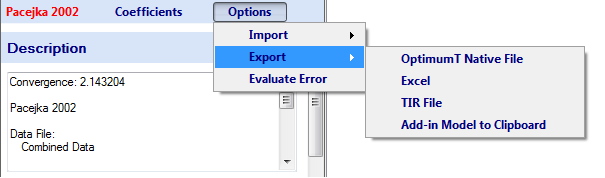
\includegraphics[width=1.0\textwidth]{AddinExport.png}
	\caption{Export the Encoded Model Coefficients from OptimumTire}
	\label{fig:AddinExport}
\end{figure}

The inputs and outputs of the add-in are expected to be in the coordinate system defined for the model. The syntax used for the inputs of the functions is demonstrated in the following equation.

\begin{center}
\texttt{Output = Function(Fz, SA, SR, IA, V, P, ModelCoefficients)}
\end{center}

The coordinate system can be queried using the command:
\begin{center}
\texttt{GetModelInfo(ModelCoefficients)}
\end{center}

The units used are also restricted. The units used are displayed in Table~\ref{tbl:AddinUnits}. The values calculated are outputted in the same units as those in the table.

\begin{center}
\begin{longtable}{|c|c|}
			
			\hline
			\multicolumn{2}{|c|}{\cellcolor{tblue}\textbf{Add-in Units}} \\ \hline
			\rowcolor{ttblue}\textbf{Inputs} & \textbf{Unit} \\ \hline
			Normal Load (Fz) &Newton \\ \hline
			Inclination Angle (IA)	&degree \\ \hline
			Slip Angle (SA)	&degree \\ \hline
			Slip Ratio (SR)	&ratio \\ \hline
			Speed (V)	&meter/sec \\ \hline
			Pressure (P)	&bar \\ \hline
			\hline
											
			\caption{Units used in the OptimumTire Add-in}
			\label{tbl:AddinUnits}
			
\end{longtable}
\end{center}

\subsection{Using the Add-in with Excel}
\label{sec:OptimumTAddin:Excel}

The installation and use of the add-in in Excel 2007 will be demonstrated. Once OptimumTire is installed the Add-in can be accessed easily from Excel. First the user should click the \textit{Start} button in the top left corner of Excel. Then click the \textit{Excel Options} button as shown in Figure~\ref{fig:ExcelOptions}.

\begin{figure}[H]
	\centering
		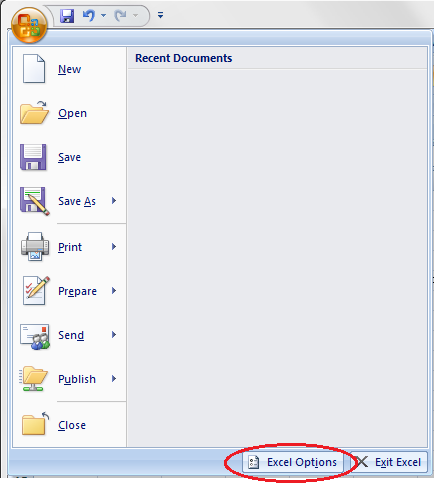
\includegraphics[width=.75\textwidth]{ExcelOptions.png}
	\caption{Excel Options}
	\label{fig:ExcelOptions}
\end{figure}

Once the Excel options are open click on \textit{Add-Ins} on the left side of the window. In the dropdown box labeled \textit{Manage:} near the bottom of the window select \textit{Excel Add-ins}. This is shown in Figure~\ref{fig:ExcelAddins} Then click on the \textit{Go} button. 

\begin{figure}[H]
	\centering
		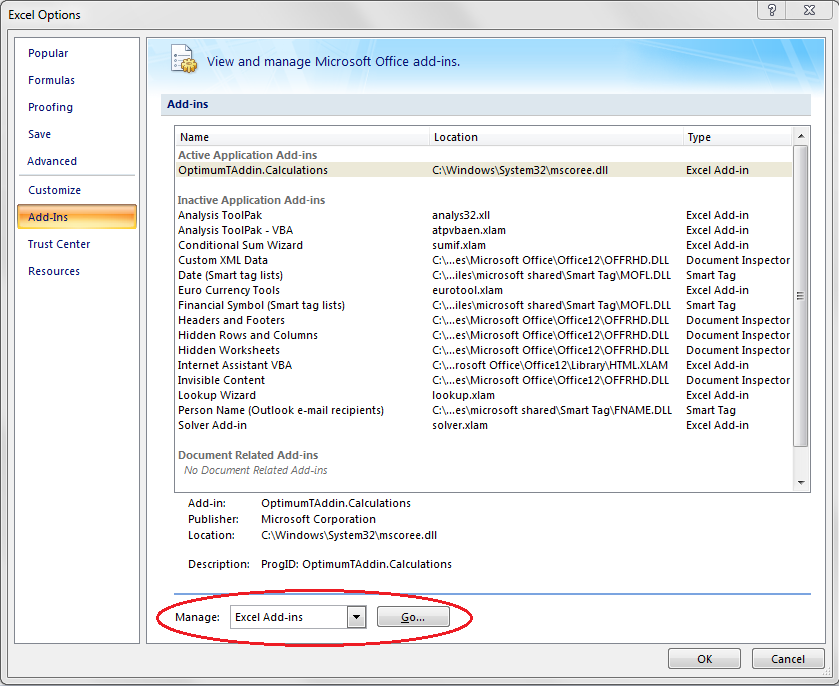
\includegraphics[width=1.0\textwidth]{ExcelAddins.png}
	\caption{Excel Add-Ins}
	\label{fig:ExcelAddins}
\end{figure}

\begin{figure}[H]
	\centering
		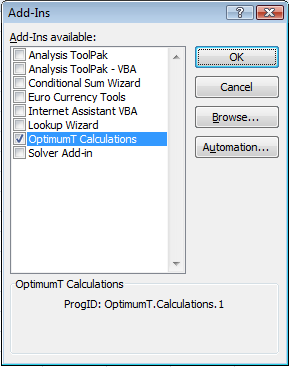
\includegraphics[width=.4\textwidth]{ImplementingAddin.png}
	\caption{Implementing the OptimumTire Add-In}
	\label{fig:ImplementingAddin}
\end{figure}


The \textit{Add-ins} selection window will now appear. In Figure~\ref{fig:ImplementingAddin} \textit{OptimumT.Calculations} is shown in the list of add-ins. This add-in will have to be added to list by clicking on the button labeled \textit{Automation...}. This will open the \textit{Automation Server} window as shown in Figure~\ref{fig:AutomationServer}. Selecting \textit{OptimumT.Calculations} and pressing the \textit{OK} button will load the COM add-in into Excel. Now the add-in can be used in the same way as functions built into Excel.

\begin{figure}[H]
	\centering
		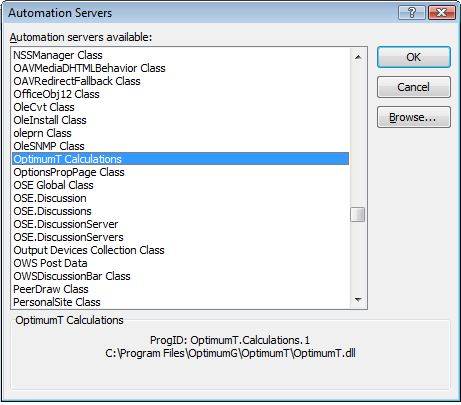
\includegraphics[width=.9\textwidth]{AutomationServer.png}
	\caption{Selecting the COM Add-in in Excel }
	\label{fig:AutomationServer}
\end{figure}


Now the Add-in can be used in Excel by clicking on the \textit{Insert Function} button in Excel. This will open the window shown below in Figure~\ref{fig:InsertFunction}. The available functions will be displayed by selecting \textit{OptimumTExcelAddin} in the categories dropdown box.

\begin{figure}[H]
	\centering
		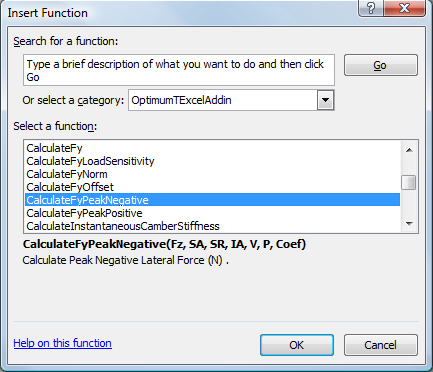
\includegraphics[width=.8\textwidth]{InsertFunction.png}
	\caption{Inserting OptimumTire Functions into Excel}
	\label{fig:InsertFunction}
\end{figure}

Then the parameters of the function can be inputted as shown in Figure~\ref{fig:AddinResults}. As can be seen in this figure the input parameters are the six tire model inputs (normal load, slip angle, slip ratio, inclination angle, velocity and inflation pressure) and the tire model coefficients. The tire model coefficients are inputted as an encoded string as shown in Figure~\ref{fig:AddinEncodedCoefficient}.

\begin{figure}[H]
	\centering
		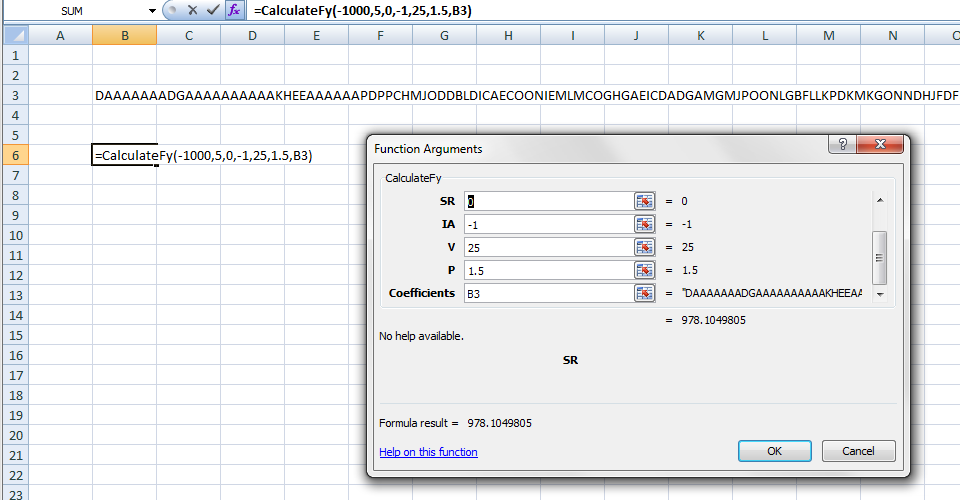
\includegraphics[width=1.0\textwidth]{AddinResults.png}
	\caption{OptimumTire Add-in Input Parameters}
	\label{fig:AddinResults}
\end{figure}

\begin{figure}[H]
	\centering
		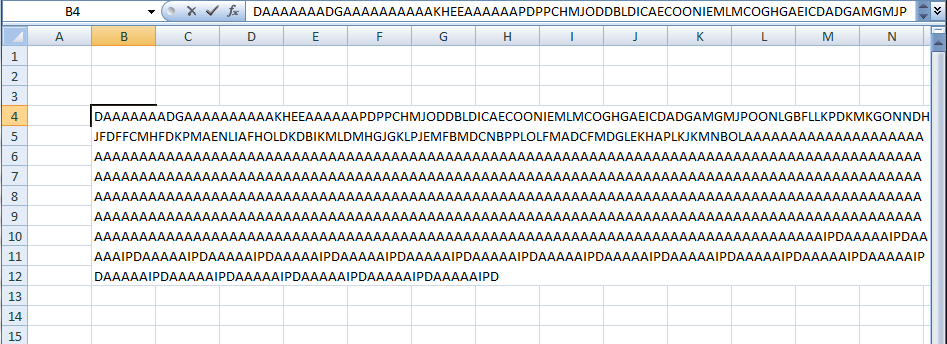
\includegraphics[width=1.0\textwidth]{AddinEncodedCoefficient.png}
	\caption{Encoded String that represents the Model Coefficients}
	\label{fig:AddinEncodedCoefficient}
\end{figure}


\subsection{Matlab COM Add-in}
\label{sec:OptimumTAddin:COMMatlab}

The use of the COM add-in in Matlab is demonstrated in this section. Every time that Matlab is opened the add-in needs to be loaded. The add-in is loaded in Matlab using the \textit{actxserver} function as shown below in Figure~\ref{fig:MatlabAddin}. Then all of the add-in functions can be accessed through the \textit{handle.method} syntax, were \textit{handle} is the variable that the add-in was loaded as and \textit{method} is the OptimumTire function that is to be used. In the figure below \textit{example} is the handle and \textit{GetLicense}, \textit{CalculateFy} and \textit{CalculateCorneringStiffness} are all functions. To get the full list of the available functions just type \textit{handle.Methods} in the Matlab command window.

\begin{figure}[H]
	\centering
		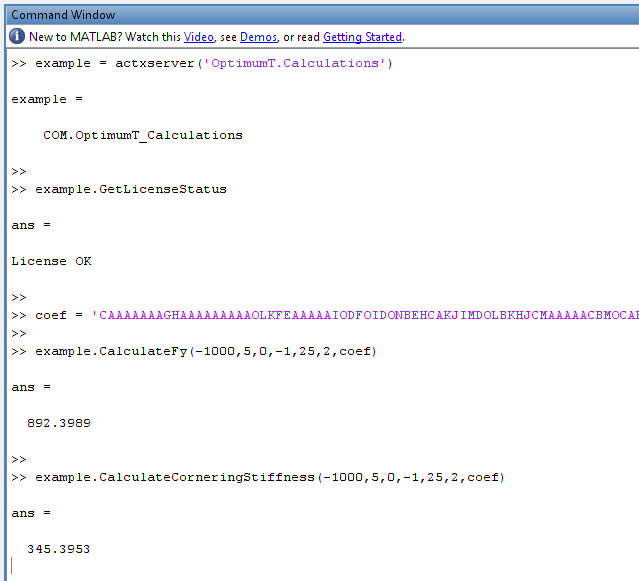
\includegraphics[width=1.0\textwidth]{MatlabAddin.png}
	\caption{Using the OptimumTire Add-in in Matlab}
	\label{fig:MatlabAddin}
\end{figure}

An example of the add-in being used in a m-file is shown in Figure~\ref{fig:mfileAddin}. In this example the handle variable(h in this case) is checked to see if it exists. If it does not exist then it loads the add-in. If it does already exist the add-in is not reloaded. This Matlab m-file is also included with OptimumTire. It is located in the \textit{Documents} folder of the user who installed OptimumTire in a folder called \textit{Matlab COM Addin}.

\begin{figure}[H]
	\centering
		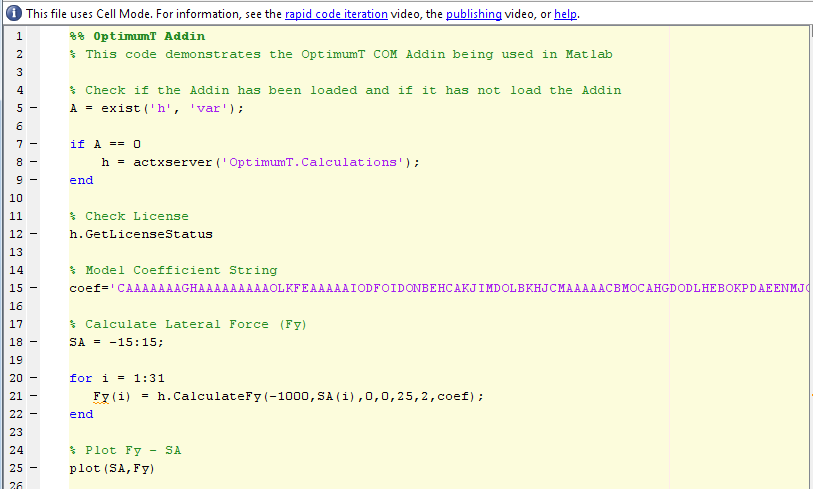
\includegraphics[width=1.0\textwidth]{mfileAddin.png}
	\caption{Using the OptimumTire Add-in in a Matlab m-file}
	\label{fig:mfileAddin}
\end{figure}

\subsection{Using the COM Addin in Programs}
\label{sec:OptimumTAddin:ComProgram}

The exact method for using the OptimumTire add-in with your own programs will depend on your programming environment. Please refer to the documentation that supplied with your programming environment for details on using COM components.

In most environments, you will need to add a reference to the OptimumTire type library. This is called \texttt{OptimumT 1.0 Type Library} or \texttt{OptimumTLib}.

There is an example C\# project provided with OptimumTire. It is located in the \textit{Documents} folder of the user who installed OptimumTire in a folder called \textit{OptimumTAddinExample}. The main function for this program is:


\begin{verbatim}
static void Main(string[] args)
{

    Console.WriteLine("Welcome to the OptimumTire Add-in example program\n\n");
           
    string modelCoef = "CAAAAAAAGHAAAAAAAAPELJFMGGGGGKODAAAAAKBEAJGPMLPDA" +
        "JJIEFPLNLHAAAODEGJIGBAMFAOJCLPLOLKEMCNLBODPFNNLKNOLOEODEF" +
        "BFFFBEJBLJCLPDHLONLLMDKFOAJHKDPGDCEELLNIHNCOMLODBJIJLLCMD" +
        "NJANDAKBPFDPLGJNNGIPLIMNKOJPDICBKMHPDEJDNMMNLGAODMDAMNELK" +
        "NMNDFJJCPJLDLNEJGILLNMHPLIBMDMNBAOBEOFBKBLPDLPFNCKILEHLCC" +
        "JKDNIBOCJIDBPNDMILDPDGNMABEDPBOJOAMMFEBCJPDOIFECOKDDMPDCO" +
        "MDCHNCOIOLKKJGMEBEFCJCBCBEMIMFMFLDFAGGKHPDMGNFBGMDMDANLHM" +
        "DKPIHEKKLABLCAEODKNGEIIAEJHMKKBAEBGKBANOLOHEJBDCMHFOFEJPL" +
        "KFAGCFMLAAAAAAAAAAAAAAAAAAAAAAAAAAAAAAAAAAAAAAAAAAAAAAAAA" +
        "AAAAAAAAAAAAAAAAAAAAAAAAAAAAAAAAAAAAAAAAAAAAAAAAAAAAAAAAA" +
        "AAAAAAAAAAAAAAAAAAAAAAAAAAAAAAAAAAAAAAAAAAAAAAAAAAAAAAAAA" +
        "AAAAAAAAAAAAAAAAAAAAAAAAAAAAAAAAAAAAAAAAAAAAAAAAAAAAAAAAA" +
        "AAAAAAAAAAAAAAAAAAAAAAAAAAAAAAAAAAAAAAAAAAAAAAAAAAAAAAAAA" +
        "AAAAAAAAAAAAAAAAAAAAAAAAAAAAAAAAIPDAAAAAIPDAAAAAIPDAAAAAA" +
        "AAAAAAAIPDAAAAAIPDAAAAAIPDAAAAAIPDAAAAAIPDAAAAAIPDAAAAAIP" +
        "DAAAAAIPDAAAAAIPDAAAAAIPDAAAAAIPDAAAAAIPDAAAAAIPDAAAAAIPD" +
        "AAAAAIPDAAAAAIPDAAAAAIPDAAAAAIPDAAAAAIPDAAAAAIPDAAAAAIPD";

    OptimumTLib.Calculations calc = new OptimumTLib.Calculations();

    // Display the type of model and the coordinate system
    Console.WriteLine("The model is:");
    Console.WriteLine(calc.GetModelInfo(modelCoef));


    // set up variables to plug into the tire model
    float Fz = -3000.0f;    // the vertical load [N]
    float IA = 1.0f;        // the inclination angle [deg]
    float SR = 0.0f;        // the slip ratio [fraction]
    float V = 10;           // the speed [m/s]
    float P = 2;            // the inflation pressure [bar]

    // declare a variable to store the calculated lateral force in
    float Fy;
            
    Console.Write("\n\n   SA      Fy\n");
    // loop through a series of slip angles and display the resulting force
    for (float SA = -10.0f; SA <= 10.0f; SA+=2.0f)
    {
        Fy = calc.CalculateFy(Fz, SA, SR, IA, V, P, modelCoef);
        Console.WriteLine(string.Format("{0,5} {1,10}", SA, Fy));
    }

    Console.Write("\nPress any key to exit...");
    Console.ReadKey();
}
\end{verbatim}

			
\section{Template Manager}
\label{sec:TemplateManager}

The template manager allows the user to easily organize or delete templates in OptimumTire. The template manager can be accessed by clicking on \textsl{Advanced} in the main toolbar and then clicking on \textsl{Template Manager}. A window similar to that shown in Figure~\ref{fig:TemplateManager} will open. In this window the user can manage graph templates, CSV import templates, coefficient boundaries and model export templates by clicking on the associated tabs. As can be seen in the figure the coefficient boundaries are organized by the different models. The models can be chosen from the dropdown box above the list of templates top of the window.

\begin{figure}[H]
	\centering
		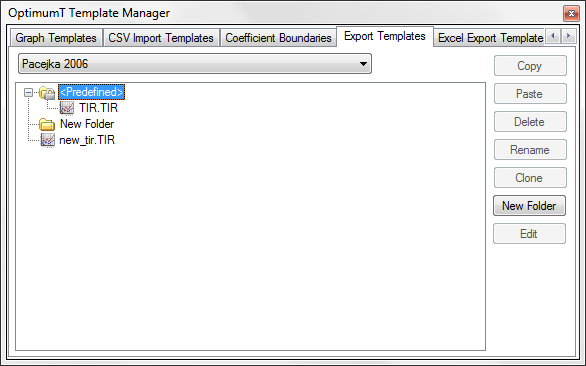
\includegraphics[width=1.0\textwidth]{TemplateManager.png}
	\caption{Template Manager}
	\label{fig:TemplateManager}
\end{figure}

The templates can be deleted, renamed, or cloned using the buttons on the right side of the \textsl{Template Manager}. New folders can also be created so that the templates can be easily organized. The templates that are contained in the \textsl{Predefined} folder are included in OptimumTire and cannot be edited or deleted. However they can be cloned. When they are cloned the copied version of the template will be moved outside of the \textsl{Predefined} folder, so that it can be modified. The paste button allows the user to paste files from the clipboard into the appropriate folder which a useful feature when transfering large numbers of templates.

\section{Project Backups}
\label{sec:ProjectBackups}

OptimumTire saves a backup of the project before each save operation. This allows you to recover from a corrupted project or to recover if you accidentally made a unwanted change to the project and saved it. By default the last five revisions of the project are stored.

To go to a previous version of the project, click on the \textsl{Advanced} menu then on \textsl{Revert Project}. You will then see the \textsl{Revert Project} dialog (shown in Figure \ref{fig:RevertProject}). Select the backup that you wish to revert to and click on \textsl{Revert}. The date and time shown in this dialog is the time at which that version was initially created.

\begin{figure}[H]
	\centering
		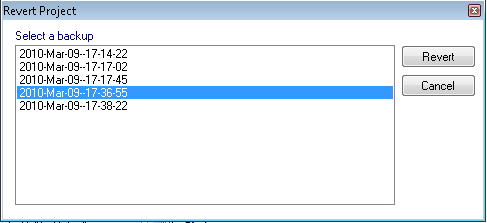
\includegraphics[width=1.0\textwidth]{RevertProject.png}
	\caption{Revert Project dialog}
	\label{fig:RevertProject}
\end{figure}

When you revert a project, OptimumTire automatically creates a backup of the project immediately before reverting it. This allows you to "undo" a revert operation.

If a project fails to load, the \textsl{Revert Project} dialog will automatically be shown. This allows you to recover your project from an earlier backup.

\section{Error Evaluation}
\label{sec:ErrorEvaluation}

The \textsl{Error Evaluation} tool is shown in Figure~\ref{fig:ErrorEval}. This tool allows quick comparison of the error of the tire models against different sets of raw data. It also allows comparison between the four different types of error calculation. To access this tool first select the tire model for the error to be evaluate on in the project tree. At the top of the data entry form select \textsl{Options} and then \textsl{Evaluate Error}.

Once the \textsl{Error Evaluation} is open the data to be compared should first be selected in the list on the left. Then the models to base the error calculation should be selected. Clicking on the \textsl{Evaluate} button at the bottom of the window will calculate and display the error each of the different error calculation methods. 

\begin{figure}[H]
	\centering
		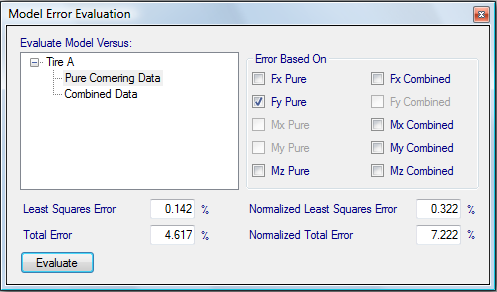
\includegraphics[width=1.0\textwidth]{ErrorEval.png}
	\caption{Error Evaluation}
	\label{fig:ErrorEval}
\end{figure}

\section{Lookup Table Export}
\label{sec:LookupTableExport}
OptimumTire offers the possibility to export lookup tables. These tables are compatible with simulation products such as CarSim or other software that uses a lookup table for modelling tyre performance rather than directly importing model coefficients and equations.
Lookup tables may be exported by selecting a model to export from the tree then clicking ~\textsl{Options->Export->Lookup table}. This will bring up the lookup table export form shown below.

\begin{figure}[H]
	\centering
		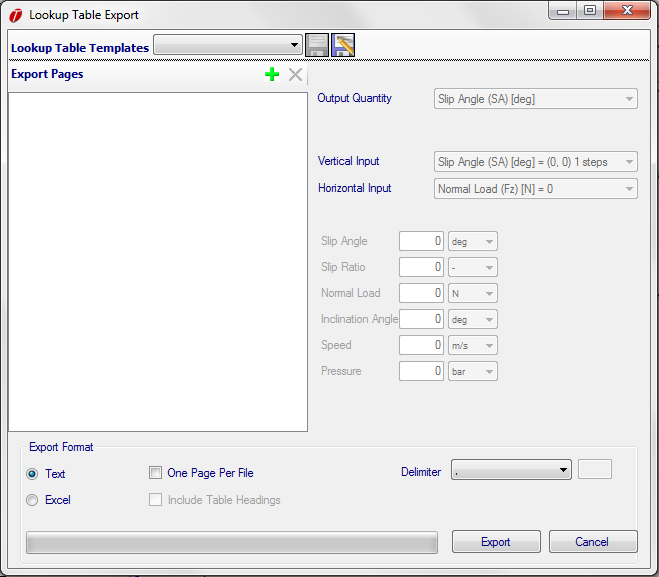
\includegraphics[width=1.0\textwidth]{LookupExportForm.png}
	\caption{Lookup Table Export Form}
	\label{fig:LookupExportForm}
\end{figure}

The form is split into three parts. The first is the \textsl{Page Tree}. Pages can be added to the export file by clicking the green \textsl{plus} sign and deleted by clicking the red \textsl{cross}. Pages may also be renamed in the tree, these names will provide the basis for the file names when exporting text files, or the sheet names when exporting to Excel. 

\begin{figure}[H]
	\centering
		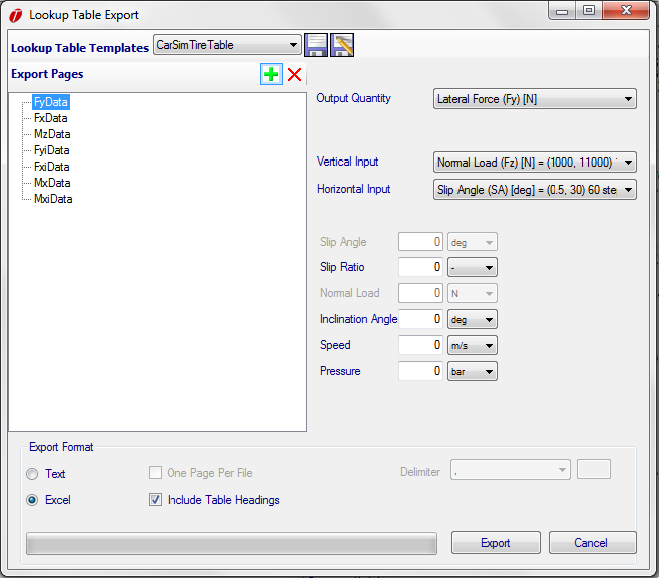
\includegraphics[width=1.0\textwidth]{LookupExportFormPopulated.png}
	\caption{Lookup Table Export Settings}
	\label{fig:LookupExportFormPopulated}
\end{figure}

The second part of the form is the \textsl{Output Settings}. Each page in the page tree has an individual output settings sheet which specifies the parameters of the look up table. The output dropdown specifies which OptimumTire output will be used to populate the table. The \textsl{Vertical} and \textsl{Horizontal} dropdowns allow you to specify the type, range and step of the vertical and horizontal axes. The remaining boxes specify the values of the outputs to be held constant in the table.

The third part of the table is the \textsl{Format section}.  This specifies the global format for the export. Files may be exported as an MS Excel workbook or as text file. Text files may export multiple pages in one file or export each page to an individual file by selecting the \textsl{one page per file radio button}. When exporting files to excel a labels may be added to the tables to indicate the names of the table parameters. This is done by selecting the \textsl{Include Table Headings check box.} The text file delimiter may be adjusted using the delimiter drop down or a custom delimiter may be used by typing a delimiter in the \textsl{custom delimiter text box.}

A useful feature of the lookup table export is the ability to save the settings in a template for repeated exports. The \textsl{lookup table template bar} is located at the top of the form.  Templates may be applied using the dropdown menu or new templates saved using the save icons.

\chapter{Tips and Tricks}
\setcounter{figure}{0}
\setcounter{table}{0}

\label{sec:TipsandTricks}
\section{Plot All Data}
\label{sec:PlotAllData}
By default when raw data is inputted into OptimumTire the \textsl{Plot All Data} option is enabled. This option will cause all of the data to appear in graphs regardless of the graph input parameters. This allows the user to quickly view the data and check that it is correct before continuing. However the color of the graphed data will not vary with the input parameters. Therefore to look at only certain parts of the data or to have the data colored by the graphing parameters this option needs to be disabled.

There are three different ways to disable the \textsl{Plot All Data} option. The first one is by right clicking on the raw data in the project tree and selecting \textsl{Remove "Plot All Data" In All Graphs}. This is shown in Figure ~\ref{fig:PlotAllData}. This will disable the feature for the selected data set in all of the graphs.

\begin{figure}[H]
	\centering
		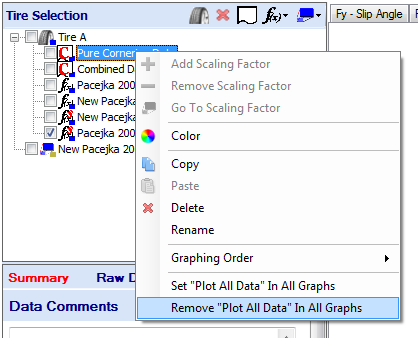
\includegraphics{PlotAllData.png}
	\caption{Plot All Data Option in the Project Tree}
	\label{fig:PlotAllData}
\end{figure}

The other two procedures to disable this option are located in the Project Items Setup at the bottom of the graph setup form as shown in Figure~\ref{fig:PlotAllDataOption}. Since this is located in the graph setup form it will only affect the graph that it corresponds to. As can be seen \textsl{"<all data>"} will appear to the right of the name of the data if \textsl{Plot All Data} is enabled. By right clicking on the data and clicking on the \textsl{Plot All Data} selects or unselects this feature. The Options button in the upper right of the figure allows the user to set all or no items to \textsl{Plot All Data}. Again this will change all of the items for the current graph only. 

\begin{figure}[H]
	\centering
		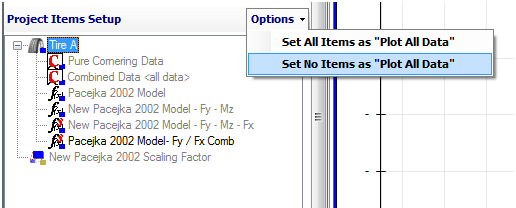
\includegraphics{PlotAllDataOption.png}
	\caption{Plot All Data Option in the Project Item Setup}
	\label{fig:PlotAllDataOption}
\end{figure}

\section{Large Tolerance Graph Inputs}
\label{sec:LargeToleranceGraphInputs}
There are cases when you want to make graphs without regard to a certain tire condition. For example, if you want to plot data for several different inflation pressures, without typing in all of the specific pressures into the display. In cases like this, you can simply set the graph input as some arbitrary fixed value and set a very large tolerance. Taking the inflation pressure example, if you had tire data taken at 1.50, 1.75, 2.00 and 2.25 bar, you could set the graph input for inflation pressure to a fixed value of 2.00 bar and set the tolerance to 2.00 bar. All of the inflation pressures will then be displayed.

\section{Override Default Name in Legend}
\label{sec:OverrideDefaultNameinLegend}
Often the name of an item (a tire model or raw data) will be too long to conveniently view in the legend. Therefore you can easily display a custom name in the legend without having to change the name of the item. This is done by clicking on the item in the project tree that a custom name is to be given to. In the data entry area the input form of the selected item will appear as shown in Figure~\ref{fig:LegendName}. The custom legend name will be used if the checkbox labeled \textsl{Override default name} in legend is checked. The custom name can be inputted into the textbox below the textbox below. The resulting graph with the custom legend name can be seen in Figure~\ref{fig:CustomLegendNames}.

\begin{figure}[H]
	\centering
		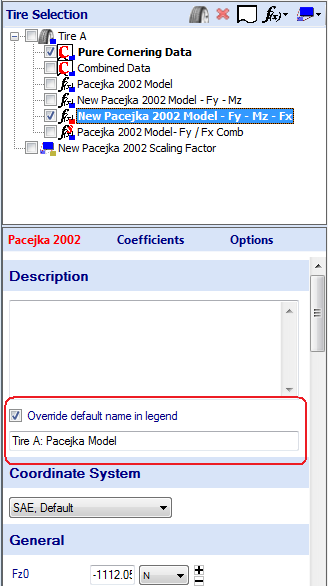
\includegraphics{LegendName.png}
	\caption{Override Default Name in Legend}
	\label{fig:LegendName}
\end{figure}

\begin{figure}[H]
	\centering
		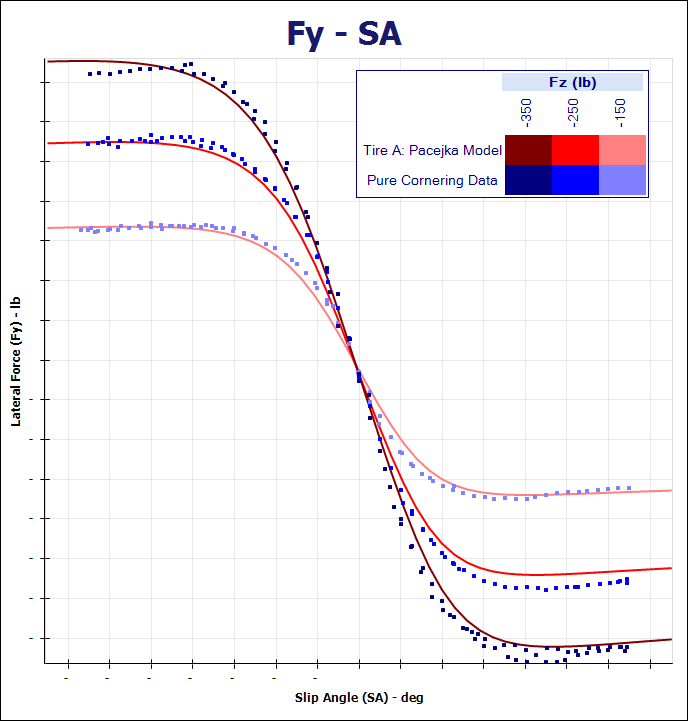
\includegraphics[width=1.0\textwidth]{CustomLegendNames.png}
	\caption{Custom Tire Model Name}
	\label{fig:CustomLegendNames}
\end{figure}

\section{Changing Units}
\label{sec:ChangingUnits}	
When a unit is changed in OptimumTire its corresponding value is automatically converted to the new unit. If you wish to change the unit of a quantity without performing a unit conversion, hold down the \textsl{shift} key while selecting the new unit. For example, if you type 10 into an input box with the unit m selected, but you wish to enter 10\textsl{mm}, simply changing the unit to \textsl{mm} will perform a unit conversion, resulting in 10000\textsl{mm}. If you hold down the \textsl{shift} key while selecting the new unit, the desired result of 10\textsl{mm} will result.

\section{Preview Model Coefficient Change}
\label{sec:PreviewModelCoefficientChange}
The values of the model coefficients can be changed by double clicking on the "+" or "-" button next to the coefficient. If the model is shown on a graph, holding down the "+" or "-" button will show a preview of the model with the coefficient modified by 10\%. An example of this is shown in Figure ~\ref{fig:PreviewCoefChange}. In this figure the "+" button of the $pDy1$ coefficient is being held down. This change can be made permanent by double clicking on this button. 

\begin{figure}[H]
	\centering
		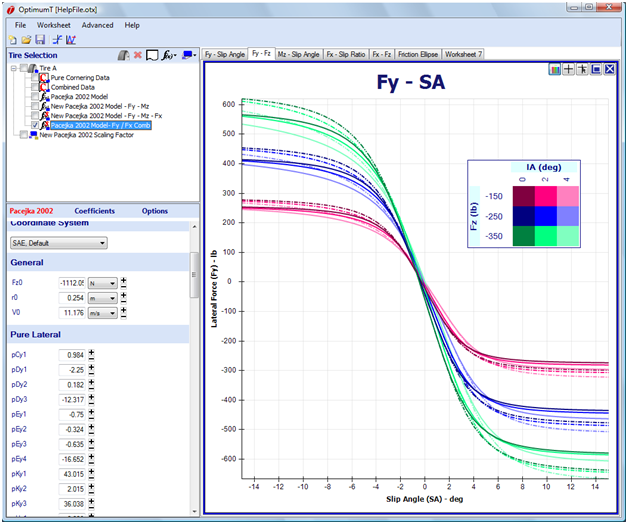
\includegraphics[width=1.0\textwidth]{PreviewCoefChange.png}
	\caption{Preview Model Coefficient Change}
	\label{fig:PreviewCoefChange}
\end{figure}

\section{Hide Axis Values}
\label{sec:HideAxisValues}
The user can choose whether or not to display axis values on the graphs. This can be very important to ensure confidentiality of the data. This option is available in the Axis Selection drop down dialog boxes as shown in Figure~\ref{fig:HideAxisValues}. If the \textsl{Hide Axis Value}s box is checked the numeric values on the specified graph axis will not be displayed. 

\begin{figure}[H]
	\centering
		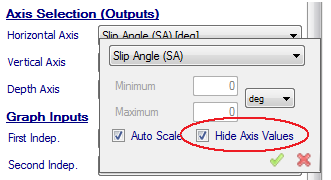
\includegraphics{HideAxisValues.png}
	\caption{Hide Axis Values}
	\label{fig:HideAxisValues}
\end{figure}


\section{Importing Multiple Data Files}
\label{sec:ImportMultipleDataFiles}
If more than one data file needs to be imported \textsl{and} merged, then they can be simply be selected together when choosing files to import. Hold down the shift or ctrl key to select multiple files. Note that all the files selected must be in exactly the same format (columns in the same order and the same units used). This feature can be useful if multiple files are produced in a single test. For example, if cornering data for different inclination angles are contained in different files, it is useful to multi-select when importing so that these files are merged within OptimumTire when they are imported.

